\section{Módulo do Chute}\label{sec:modulo_chute}

O mecanismo de chute do robô foi elaborado utilizando dois solenóides como atuadores, um responsável pelo chute para frente e outro responsável pelo chute alto. E a placa (Figura~\ref{fig:modulo_chute}) é responsável por produzir a alta tensão necessária para ativar os dois solenóides, e transmitir a energia acumulada para acionar os atuadores.

\begin{figure}
	\centering
	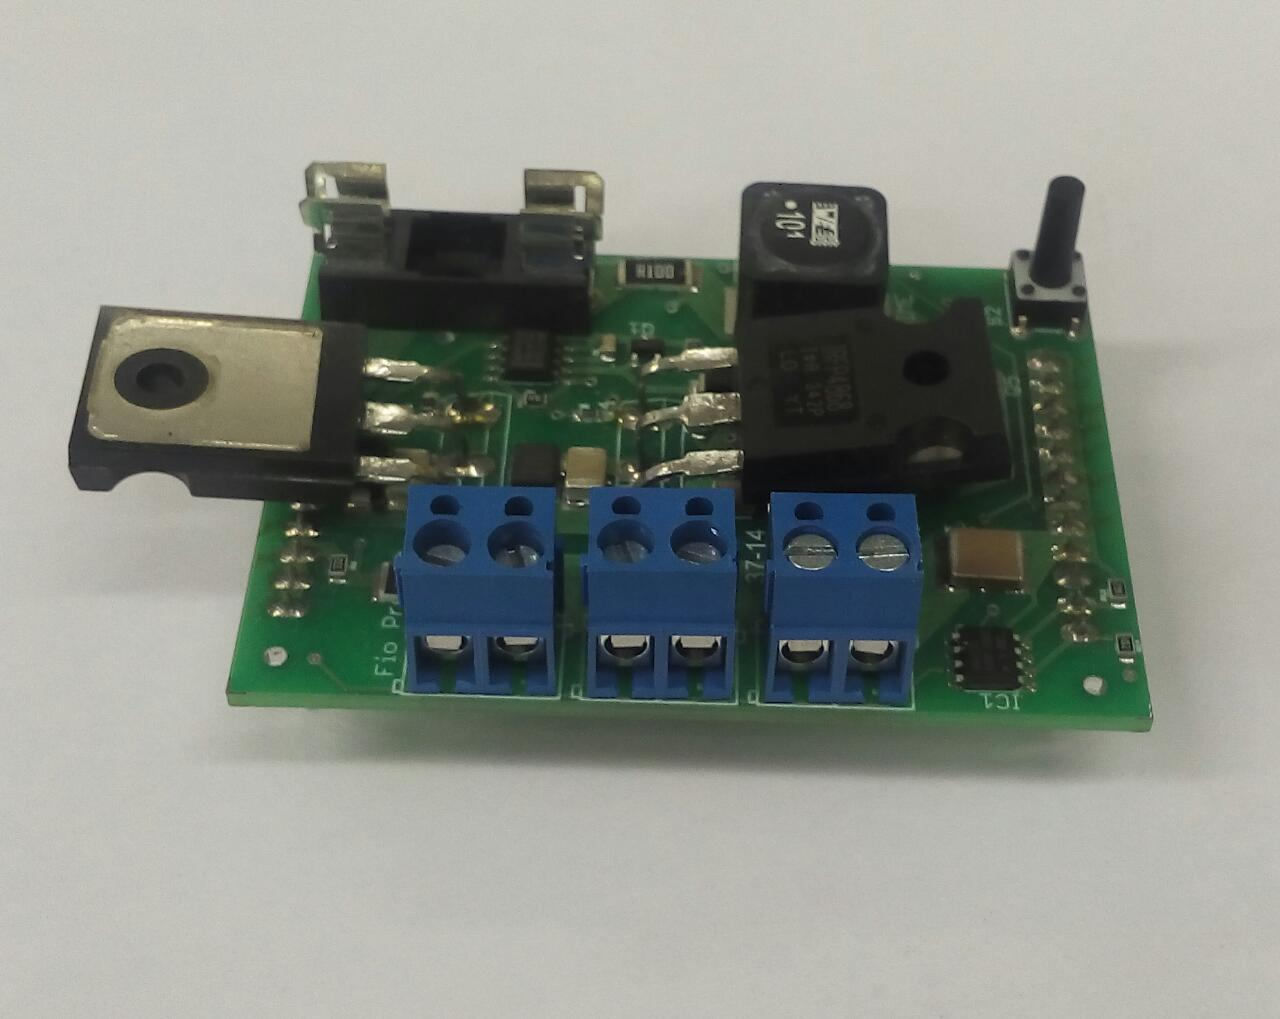
\includegraphics[scale=1]{modulo_chute}
	\caption{Módulo do Chute}
	\label{fig:modulo_chute}
\end{figure}

A placa funciona através de um circuito de conversão DC-DC controlado pelo circuito integrado MC34063 que converte os 7,8V DC da bateria em uma saída de 180V DC ligada a dois capacitores eletrolíticos de 2200 $\mu$F e 200V. Além desse circuito existe ainda um circuito para chavear a tensão dos capacitores nos solenóides, o que é feito utilizando um TC4427 driver de MOSFET e dois MOSFETs de potência IRFP4868PBF. 
O controle desse módulo é feito através da classe chute que utiliza a classe degrau unitário para limitar a energia transmitida a bola alterando a duração do intervalo de tempo que os MOSFETs ficarão ativados.

\begin{figure}
	\centering
	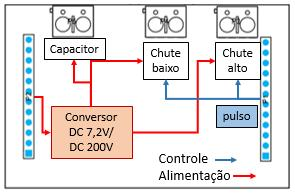
\includegraphics[scale=1]{blocos_chute}
	\caption{Diagrama de blocos do módulo de chute}
	\label{fig:blocos_chute}
\end{figure}


% vim: tw=80 et ts=2 sw=2 sts=2 ft=tex spelllang=pt_br,en
